\documentclass[twocolumn]{article}
%\documentclass{article}
\usepackage{fullpage}
% you really only need to use one of graphicx or epsfig
% there are example of using each one in this file
%\usepackage[dvips]{graphicx}
%usepackage{epsfig}
\usepackage{pgfplots}

% if you want two columns per page, but you also need to reformat the figures
% to span both columns if you do this
%\twocolumn
\begin{document}
\title{Testing Characteristics of the Linux Page Replacement Policy}

\author{Callen Rain \& Justin Cosentino}

\maketitle

\begin{abstract}
This paper describes some of the techniques used to identify the behavior of the Linux page replacement and discusses the implementation of a system call that provides page replacement statistics.  The system call provides page fault statistics for minor and major faults for a single process, processes grouped by owners, and all processes on the system. Several tests were developed that accessed large segments of memory on a Linux virtual machine. In each of the tests, access patterns exploited specific page replacement schemes and favored others. An initial hypothesis of a Least Recently Used (LRU) algorithm was partially supported, although there was some evidence that the Linux implementation is a combination of various algorithms and has some characteristics resembling a working set. 
\end{abstract}

\section{Introduction}

We began with a hypothesis that the Linux system uses a Least Recently Used (LRU) page replacement algorithm, based on our analysis of the relevant kernel code and our numerous attempts in class to approximate this algorithm.  Our first few tests confirmed that the replacement policy is more like LRU than like Most Recently Used (MRU) and First In First Out (FIFO), but our test to find some distinction between LRU and a Working Set (WS) algorithm did lean in favor of some Working Set behavior rather than strict LRU. It is evident that the Linux page replacement implementation is not strictly one of the algorithms outline in class, but rather exhibits characteristics of both WS and LRU.


\section{System Call}
Our experimental methodology relies heavily on the page fault statistics system call that we implemented for the first part of this lab. The system call reports the number of page faults for all processes in the system, all the processes being run by the owner of the current process, or just the page faults for the current process. For each of these operations, the system call reports the major faults, minor faults, and the number of processes being reported on. We collected statistics primarily on major faults, as they are the page faults that result from having to replace pages in memory. 

The system call first does normal error checking, ensuring that the pointer passed in is writable and valid, that the process or processes requested exist, and that the flag is valid. We defined the ${\tt pf\_info\_struct}$, which stores the  major faults, minor faults, and the number of associated processes, and the included flags in a header file. If the user enters a pid of -1, we used the ${\tt for\_each\_process()}$ macro to loop over all the processes, incrementing the major faults, minor faults, and number of processes for each one. We then fill the fields of the included struct. If the pid is positive, we check the inputted flag. If the flag is ${\tt PGFLTSTAT\_PROC}$, we do the same procedure for just the current process. If the flag is ${\tt PGFLTSTAT\_OWNER}$, we look for the owner id of the current process, and loop through all the processes again, collecting data only for the ones that share the uid. Once completed, this information is written to the provided ${\tt pf\_info\_struct}$. 

\section{Methodology}
\subsection{Experiments}

We carried out four experiments, all contained as subroutines within one file ({\tt mem.c}). The program selects one of the subroutines from a command line argument. In every test, the Virtual Machine was configured to have $256$MB of physical memory and $128$ buckets of unsigned ints (4B) were allocated. Thus each bucket had 4MB of data contained with it. Depending on the availability of memory after the boot, the system could hold slightly less than 64 of these buckets. We used this fact to plan some of our tests and memory access patterns. 

Each test (except the random LRU test) involves two cases. In either case for a specific test, the system does roughly the same allocation routine with a slightly different final phase. In these last phases, we attempted to exploit some characteristic of the page replacement algorithm. In one case, we would access memory that we predicted would be replaced by the algorithm, and in the other case, we would access memory that we guessed had not been replaced. By printing out major fault statistics between the phases, we could get an idea of whether our hypothesis was correct or not by calculating the average page faults for each phase.  We report this average over the number of trials and include the standard deviation as a measure of the error. 

\subsubsection{Ruling Out Most Recently Used}
As discussed in class, the Most Recently Used (MRU) strategy is often a poor choice for a page replacement algorithm. Since there are only a few application specific cases in which this algorithm works well and Linux handles such a diverse workload, we hypothesize that MRU is not used as Linux's page replacement policy.

We test this hypothesis by running each case of the first experiment in file {\tt mem.c}. In both cases, this subroutine first writes 128 4MB buckets to a block of memory, which is significantly larger than what can fit in RAM. We now access a small chunk (8-12 buckets) of this large block in one of two ways. In the first case, we read in the last 12 buckets. Were the Linux page replacement policy a MRU algorithm, we would expect these memory accesses to cause major page faults as recently-used page entries would be evicted once the page table filled up. On the other hand, were the page replacement policy strictly LRU, we would expect these entries to still be within the page table and minimal major page faulting. As seen in Figure 1 and Table 1, this experiment resulted in very few major page faults, supporting our hypothesis that MRU is not used as Linux's page replacement policy.

In the second case, we read in the first 8 buckets of the large block of memory. Were the Linux page replacement policy a MRU algorithm, we would expect these memory accesses to cause very few major page faults as these least recently-used page entries would be less likely to be evicted than their recent counterparts. Conversely, were Linux page replacement policy a LRU algorithm we would expect major page faults to occur as these least recently-used entries would have been evicted once the page table filled up. The number of major page faults that occurred in this case, as depicted in Figure 1 and Table 1, were nearly an order of magnitude greater than those that occurred in the first case, further supporting our initial hypotheses. Not only does this experiment refute the possibility that Linux implements a MRU page replacement algorithm, but the displayed behavior implies an LRU implementation.  

%--------------------------------------------%

\begin{figure}[h!]
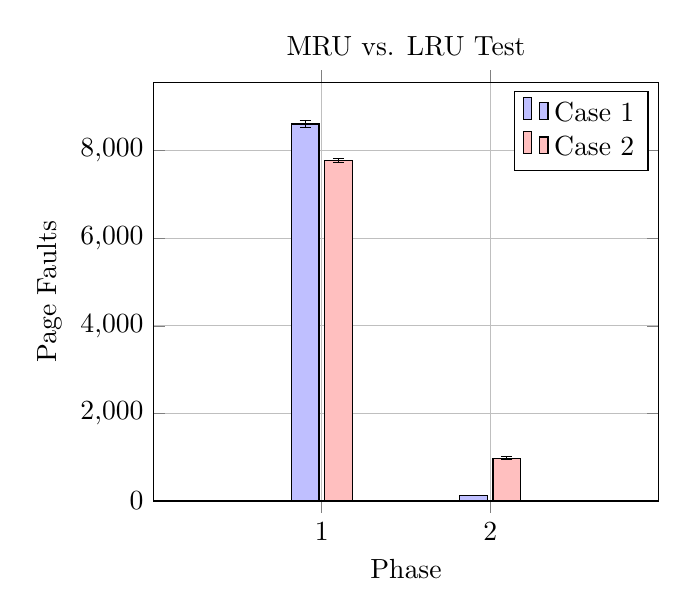
\begin{tikzpicture}
\begin{axis}[
    title = {MRU vs. LRU Test},
    width=8cm,
    xtick={1,...,2},
    xticklabels={1,2,3,4},
    grid=major,
    ybar, 
    bar width=10pt, 
    ylabel=Page Faults, 
    xlabel=Phase, 
    ymin=0, 
        enlarge x limits={abs=1}
    ]

\addplot[
    fill=blue!25,
    error bars/.cd,
        y dir=both,
        y explicit
] 
table [y error=error] {
x   y           error    label
1   8608.00 86.23 1
2   128.00 3.87 2
};

\addplot[
    fill=red!25,
    error bars/.cd,
        y dir=both,
        y explicit
] 
table [y error=error] {
x   y           error    label
1   7775.00   41.76 1
2   978.00   32.60 2
};
\legend{Case 1,Case 2}
\end{axis}
\end{tikzpicture}
\end{figure}

\begin{table}[h!]
\begin{center}
\begin{tabular}{|c|c|r|r|}
\hline
{\bf Phase } & {\bf Case} & {\bf Page Faults} & {\bf Error } \\
\hline
1 & 1 & 8608.00 & $\pm$ 86.23 \\
& 2 & 7775.00 & $\pm$ 41.76 \\
\hline
2 & 1 & 128.00 & $\pm$ 3.87 \\
& 2 & 978.00 & $\pm$ 32.60 \\
\hline
\end{tabular}
\caption{ \label{rawio} MRU versus LRU test data
{\em  Description DescriptionDescriptionDescriptionDescription  }}
\end{center}
\end{table}

%--------------------------------------------%

\subsubsection{Ruling Out First In First Out}
Given that First In First Out (FIFO) page replacement policies do not take into account memory usage information and results in B�l�dy's anomaly, we hypothesize that Linux does not make us of a FIFO based algorithm. We confirm this hypothesis by running the second subroutine in our experiment file. In both cases of this experiment, the application first writes 128 4MB buckets to a block of memory and then repeatably reads and writes to the first 8 buckets. Next, the application writes to the last 8 buckets once, effectively removing the first 8 buckets if Linux utilizes a FIFO algorithm. In the first case, this subroutine then reads the first 8 buckets. Were the Linux page replacement policy a FIFO algorithm, we would expect these read operations to major page fault, as they were the first entries related to this memory block to be added to the page table and would have been removed after the last write. On the other hand, if it is an LRU implementation we would expect minimal page faults to occur as this memory was recently accessed. As seen in Figure 2 and Table 2, no major page faults occurred, supporting our hypothesis and further strengthening our claim that Linux implements an LRU page replacement algorithm.

In the second case, the last phase of this application reads buckets 8-16. We would expect a FIFO algorithm not to page fault when performing these operations, as these buckets would not yet have been evicted from the page table. In reality, these operations resulted in nearly 1000 major page faults. This case also implies that the Linux page replacement algorithm is not a FIFO based algorithm. 
 
%--------------------------------------------%
\begin{figure}[h]
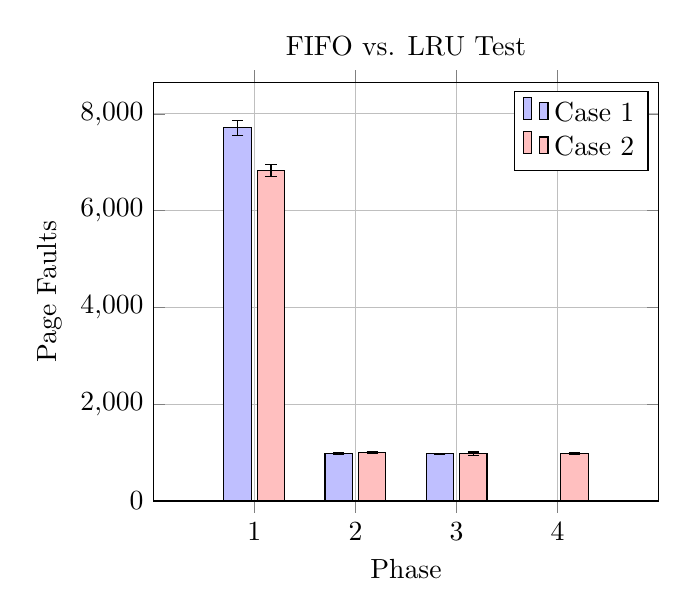
\begin{tikzpicture}
\begin{axis}[
    title = {FIFO vs. LRU Test},
    width=8cm,
    xtick={1,...,4},
    xticklabels={1,2,3,4},
    grid=major,
    ybar, 
    bar width=10pt, 
    ylabel=Page Faults, 
    xlabel=Phase, 
    ymin=0, 
    enlarge x limits={abs=1}
    ]

\addplot[
    fill=blue!25,
    error bars/.cd,
        y dir=both,
        y explicit
] 
table [y error=error] {
x   y           error    label
1   7708.00 158.27 1
2   976.00 20.27 2
3   976.00 8.89 3
4   0.00 0.00 4
};

\addplot[
    fill=red!25,
    error bars/.cd,
        y dir=both,
        y explicit
] 
table [y error=error] {
x   y           error    label
1   6832.00   128.12 1
2   993.00   20.12 2
3   979.00   33.21 3
4   983.00   15.59 4
};
\legend{Case 1,Case 2}
\end{axis}
\end{tikzpicture}
\end{figure}

\begin{table}[h]
\begin{center}
\begin{tabular}{|c|c|r|r|}
\hline
{\bf Phase } & {\bf Case} & {\bf Page Faults} & {\bf Error } \\
\hline
1 & 1 & 7708.00 & $\pm$ 158.27 \\
& 2 & 6832.00 & $\pm$ 128.12 \\
\hline
2& 1 & 976.00 & $\pm$ 20.27 \\
& 2 & 993.00 & $\pm$ 20.12 \\
\hline
3 & 1 & 976.00 & $\pm$ 8.89 \\
& 2 & 979.00 & $\pm$ 33.21 \\
\hline
4 & 1 & 0.00 & $\pm$ 0.00 \\
& 2 & 983.00 & $\pm$ 15.59 \\
\hline
\end{tabular}
\caption{ \label{rawio} FIFO versus LRU test data
{\em  Description  }}
\end{center}
\end{table}
%--------------------------------------------%

\subsubsection{Balance Between Working Set Least Recently Used}
The first two experiments imply that Linux implements neither a MRU nor a FIFO page replacement algorithm.  

%--------------------------------------------%
\begin{figure}[h]
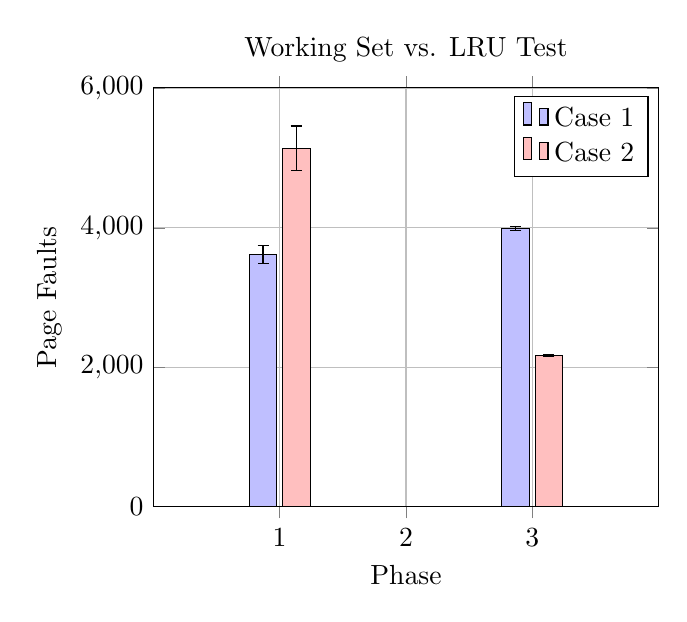
\begin{tikzpicture}
\begin{axis}[
    title = {Working Set vs. LRU Test},
    width=8cm,
    xtick={1,...,3},
    xticklabels={1,2,3,4},
    grid=major,
    ybar, 
    bar width=10pt, 
    ylabel=Page Faults, 
    xlabel=Phase, 
    ymin=0, 
    enlarge x limits={abs=1}
    ]

\addplot[
    fill=blue!25,
    error bars/.cd,
        y dir=both,
        y explicit
] 
table [y error=error] {
x   y           error    label
1   3614.00 131.24 1
2   1.00 1.00 2
3   3990.00 24.58 3
};

\addplot[
    fill=red!25,
    error bars/.cd,
        y dir=both,
        y explicit
] 
table [y error=error] {
x   y           error    label
1   5142.00   320.20 1
2   1.00   0.00 2
3   2163.00   13.96 3
};
\legend{Case 1,Case 2}
\end{axis}
\end{tikzpicture}
\end{figure}

\begin{table}[h]
\begin{center}
\begin{tabular}{|c|c|r|r|}
\hline
{\bf Phase } & {\bf Case} & {\bf Page Faults} & {\bf Error } \\
\hline
1 & 1 & 3614.00 & $\pm$ 131.24 \\
& 2 & 5142.00 & $\pm$ 320.20 \\
\hline
2& 1 & 1.00 & $\pm$ 1.00 \\
& 2 & 1.00 & $\pm$ 0.00 \\
\hline
3 & 1 & 3990.00 & $\pm$ 24.58 \\
& 2 & 2163.00 & $\pm$ 13.96 \\
\hline
\end{tabular}
\caption{ \label{rawio} Working Set versus LRU test data
{\em  Description  }}
\end{center}
\end{table}

%--------------------------------------------%

\subsubsection{Random LRU Behavior}

Main part: describe your experiments and results: For each experiment, you should:

Clearly state what your hypothesis is (i.e. "Application that does X should be a bad/good case for Linux's page replacement policy because ...)

Explain how your experiment is testing that hypothesis (We are testing this hypothesis by running application P, which does ..., N times on and collecting X,Y, and Z metrics using our system call, vmstat, time,... With these measures, we can see whether or not ... because ...).

Present your Results.

Explain your results! 
(Our results show that ... This does/does not match our expected result, because ... (if it doesn't, think about some other tests you could run to explain why it doesn't, or look for data you do have to explain it)

Quality of Experiments is much, much better than quantity; a few well thought out and well done experiments is sufficient.

\section{Conclusion}

It should include a statement of the major result(s) of your experiments (which policy(ies) is Linux's most like? and in what way(s)?). Also, tell me what you found to be the most difficult part of the hypothesis testing phase of this assignment.




\end{document}

